\section{Panduan Penyesuaian Plot dan Sintaks Matplotlib}
\label{mpltables}

\objective{
Dokumentasi Matplotlib terkadang agak sulit dijelajahi dan informasi dasar tidak selalu mudah ditemukan.
Lampiran ini meringkas dan memperagakan beberapa informasi yang paling dapat diterapkan dan berguna tentang penyesuaian plot.
Untuk pengantar Matplotlib, lihat Bab~\ref{ch:software-python}.
}

\section*{Warna} % ============================================================

Secara bawaan, setiap plot diberi warna berbeda yang ditentukan oleh ``siklus warna''.
Pengaturan ini dapat ditimpa dengan menentukan warna yang diinginkan melalui beberapa cara.
\begin{itemize}
    \item \textbf{}
\end{itemize}
Matplotlib mengenali beberapa warna dasar bawaan.

\begin{table}[H] % Basic colors.
\centering
\begin{tabular}{r|l}
    Kode & Warna \\
    \hline
    \li{'b'} & biru\\
    \li{'g'} & hijau\\
    \li{'r'} & merah\\
    \li{'c'} & sian\\
    \li{'m'} & magenta\\
    \li{'y'} & kuning\\
    \li{'k'} & hitam\\
    \li{'w'} & putih
\end{tabular}
\end{table}

Contoh berikut menunjukkan cara menerapkan warna-warna tersebut.
Hasilnya ditampilkan pada Gambar \ref{colors}.

\lstinputlisting[style=fromfile]{colors.py}

\begin{figure}  % Colors.
    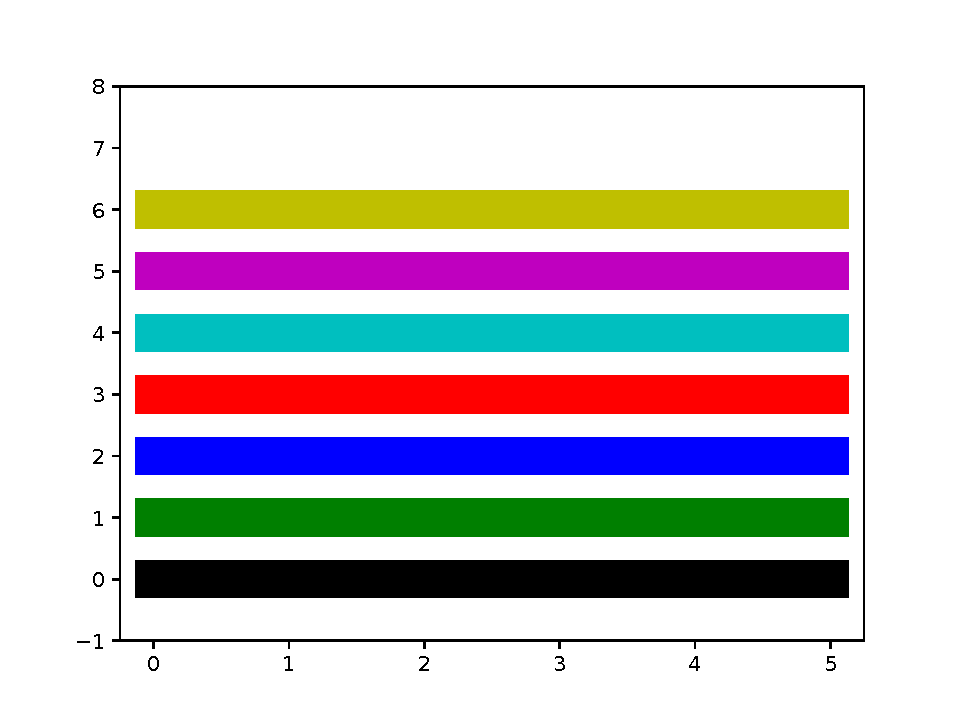
\includegraphics[width=\textwidth]{colors.pdf}
    \caption{Tampilan semua warna bawaan.}
    \label{colors}
\end{figure}

Ada banyak cara lain untuk menentukan warna.
Metode populer untuk mengakses warna yang tidak tersedia sebagai bawaan adalah menggunakan tuple \li{RGB}.
Warna juga dapat ditentukan menggunakan string heksadesimal HTML atau nama warna HTML terkait seperti \li{"DarkOliveGreen", "FireBrick", "LemonChiffon", "MidnightBlue", "PapayaWhip",} atau \li{"SeaGreen"}.

\section*{Batas Jendela} % ====================================================

Anda mungkin memperhatikan penggunaan \li{plt.ylim([ymin, ymax])} dalam kode sebelumnya. Perintah ini menetapkan batas sumbu y secara eksplisit. Demikian pula, \li{plt.xlim([xmin, xmax])} dapat digunakan untuk menetapkan batas sumbu x.
Kedua pengaturan dapat dilakukan sekaligus dengan \li{plt.axis([xmin, xmax, ymin, ymax])}.
Ingat bahwa perintah-perintah ini harus dijalankan setelah plot dibuat.

\begin{comment} % pulled this in from matplotlib lab.
\begin{table}[H]
\centering
\begin{tabular}{r|l}
    Function & Description\\
    \hline
    % \li{annotate} & adds a commentary at a given point on the plot & annotate('text',(x,y))\\
    % \li{arrow} & draws an arrow from a given point on the plot & arrow(x,y,dx,dy)\\
    % \li{axhline} & draws a horizontal line at y from xmin to xmax & axhline(y=0, xmin=0, xmax=1)\\
    % \li{axvline} & draws a vertical line at x from ymin to ymax & axvline(x=0, ymin=0, ymax=1)\\
    % \li{axhspan} & draws a rectangle from xmin to xmax and ymin to ymax, if no xmin and xmax are given it goes across the plot & axhspan(ymin, ymax, xmin=0, xmax=1)\\
    % \li{axvspan} & draws a rectangle from ymin to ymax and xmin to xmax, if no ymin and ymax are given it goes across the entire plot & axvspan(xmin, xmax, ymin=0, ymin=1)\\
    % \li{grid()} & Add gridlines\\
    \li{legend()} & Place a legend in the plot\\
    % \li{text()} & Add text at a given position on the plot\\
    \li{title()} & Add a title to the plot\\
    \li{xlim()} & Set the limits of the $x$-axis\\
    \li{ylim()} & Set the limits of the $y$-axis\\
    % \li{xticks()} & set the location of the tick marks on the x axis, returns current locations if no arguments are given\\
    % \li{yticks()} & set the location of the tick marks on the y axis, returns current locations if no arguments are given\\
    \li{xlabel()} & Add a label to the $x$-axis\\
    \li{ylabel()} & Add a label to the $y$-axis
\end{tabular}
% \caption{Some Functions to Set Plotting Options}
% \label{mpl:useful_functions}
\end{table}
\end{comment}


% BAD! plt.axis("tight") has a bug that messes with OS X on Macs.
% Another popular command is \li{plt.axis("tight")} which adjusts the axes so all data is visible and centered.

\section*{Garis} % ============================================================

\subsection*{Ketebalan} % -----------------------------------------------------

Anda mungkin memperhatikan bahwa garis-garis di atas tampak tipis, padahal kita ingin memeriksa warnanya. \li{linewidth} adalah argumen kata kunci yang secara bawaan bernilai \li{None}, tetapi dapat diberi bilangan real apa pun untuk menyesuaikan lebar garis.

Contoh berikut menunjukkan cara menerapkan \li{linewidth}.
Hasilnya ditampilkan pada Gambar \ref{linewidth}.

\lstinputlisting[style=fromfile]{linewidth.py}

\begin{figure} % Line width results
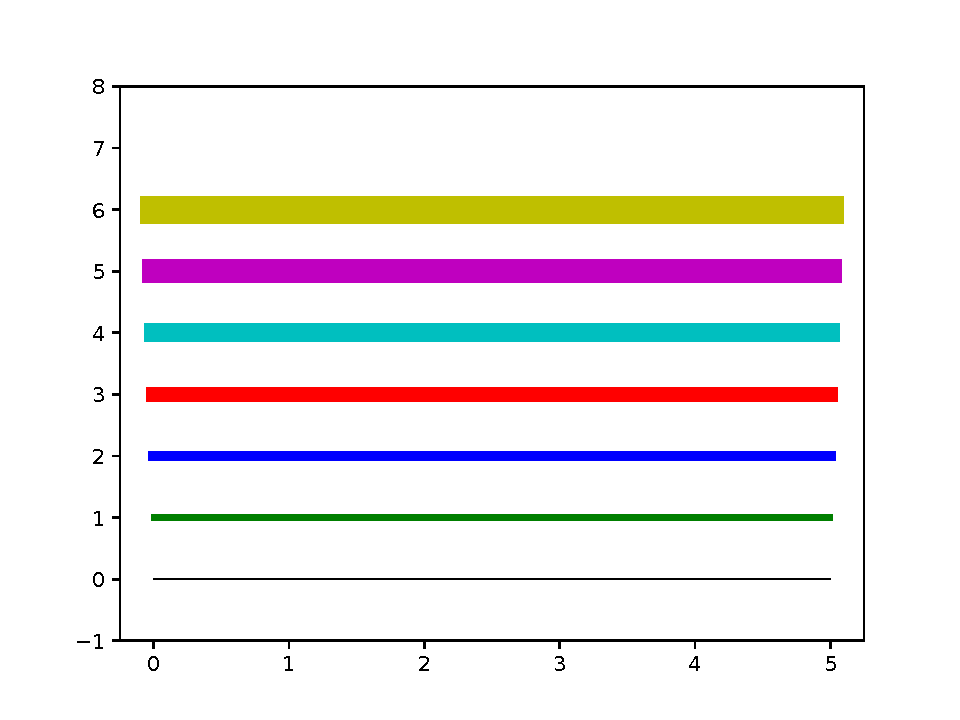
\includegraphics[width=\textwidth]{linewidth.pdf}
\caption{Plot dengan berbagai lebar garis.}
\label{linewidth}
\end{figure}

% Talk about markersize and demonstrate markers of varying sizes.

\subsection*{Gaya} % ----------------------------------------------------------

Secara bawaan, plot digambar dengan garis utuh.
Karakter string format berikut dapat digunakan untuk menunjukkan gaya garis.

\begin{table}[H] % Line style
\centering
\begin{tabular}{c|l}
    karakter & deskripsi \\
    \hline
    - & gaya garis utuh \\
    -{}- & gaya garis putus-putus\\
    -. & gaya garis setrip-titik \\
    : & gaya garis titik-titik \\
    . & penanda titik \\
    , & penanda piksel \\
    o & penanda lingkaran \\
    v & penanda segitiga\_bawah \\
    \^{} & penanda segitiga\_atas \\
    $<$ & penanda segitiga\_kiri \\
    $>$ & penanda segitiga\_kanan \\
    1 & penanda tri\_bawah \\
    2 & penanda tri\_atas \\
    3 & penanda tri\_kiri \\
    4 & penanda tri\_kanan \\
    s & penanda persegi \\
    p & penanda pentagon \\
    * & penanda bintang \\
    h & penanda heksagon1 \\
    H & penanda heksagon2 \\
    + & penanda plus \\
    x & penanda x \\
    D & penanda wajik \\
    d & penanda wajik\_tipis \\
    $|$ & penanda garis vertikal \\
    \_{} & penanda garis horizontal \\
\end{tabular}
\end{table}

Contoh berikut menunjukkan cara menerapkan \li{linestyle}.
Hasilnya ditampilkan pada Gambar \ref{linestyle}.

\lstinputlisting[style=fromfile]{linestyle.py}

\begin{figure} % Line styles
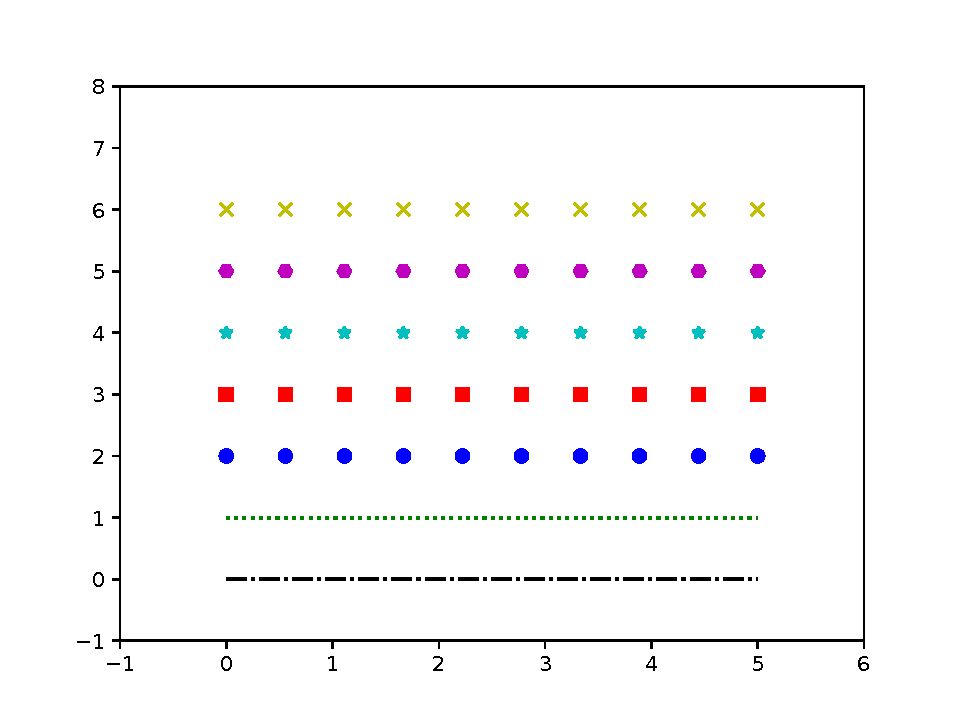
\includegraphics[width=\textwidth]{linestyle.pdf}
\caption{Plot dengan berbagai gaya garis.}
\label{linestyle}
\end{figure}

\section*{Teks} % =============================================================

Anda juga dapat menambahkan teks ke plot.
Untuk memberi label pada sumbu, gunakan \li{plt.xlabel()} dan \li{plt.ylabel()}.
Fungsi \li{plt.title()} menambahkan judul pada plot.
Jika Anda bekerja dengan subplot, perintah ini akan menambahkan judul pada subplot yang sedang diubah.
Untuk menambahkan judul di atas seluruh gambar, gunakan \li{plt.suptitle()}.

Semua perintah \li{text()} dapat disesuaikan dengan argumen kata kunci \li{fontsize} dan \li{color}.

Kita dapat menambahkan unsur-unsur ini ke contoh sebelumnya.
Hasilnya ditampilkan pada Gambar \ref{text}.

\lstinputlisting[style=fromfile]{text.py}

\begin{figure}
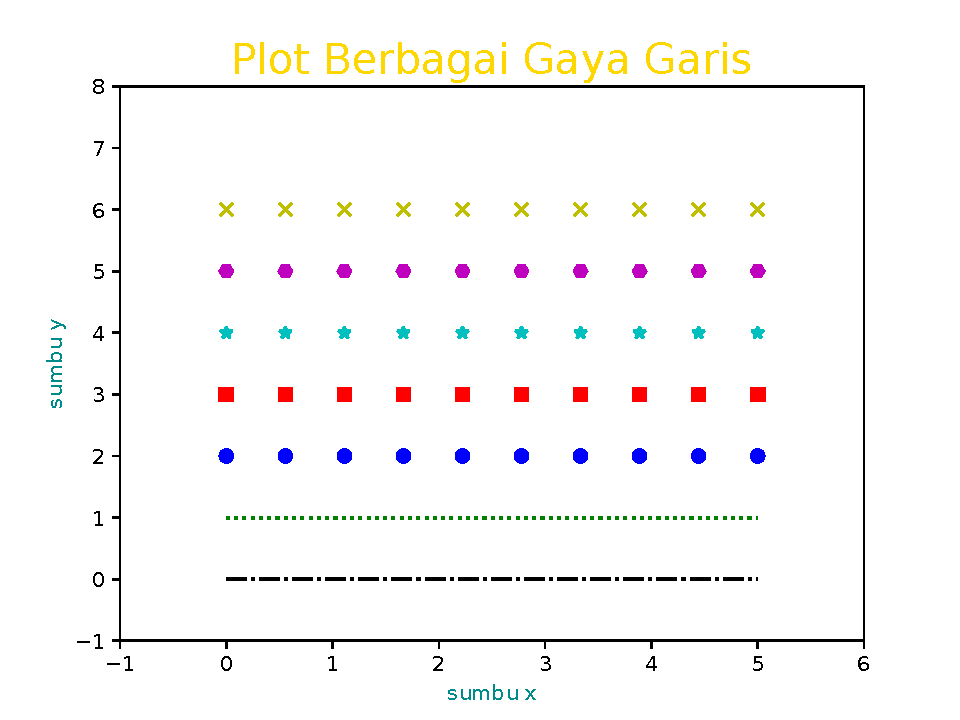
\includegraphics[width=\textwidth]{text.pdf}
\caption{Plot dengan berbagai gaya garis dan label teks.}
\label{text}
\end{figure}

\begin{comment} % PLOTTING COMMANDS
\begin{table} % Different plotting commands. Should be part of the appendix.
\centering
\begin{tabular}{|l|p{7cm}|p{3cm}|}
    \hline
    Function & Description & Usage\\
    \hline
    \li{bar} & makes a bar graph & bar(left,height)\\
    \li{barh} & makes a horizontal bar graph & barh(bottom,width)\\
    \li{fill} & plots lines with shading under the curve & fill(x,y)\\
    \li{fill\_between} & plots lines with shading between two given y
    values & fill\_ between(x,y1, y2=0)\\
    \li{hist} & plots a histogram from data & hist(data)\\
    \li{pie} & makes a pie chart & pie(x)\\
    \li{plot} & plots lines and data on standard axes & plot(x,y)\\
    \li{polar} & plots lines and data on polar axes & polar(theta,r)\\
    \li{loglog} & plots lines and data on logarithmic x and y axes &
    loglog(x,y)\\
    \li{scatter} & plots data, has more options for scatter plots than
    the plot function & scatter(x,y)\\
    \li{semilogx} & plots lines and data with a log scaled x axis &
    semilogx(x,y)\\
    \li{semilogy} & plots lines and data with a log scaled y axis &
    semilogy(x,y)\\
    \li{specgram} & makes a spectogram from data & specgram(x)\\
    \li{spy} & plots the sparsity pattern of a 2D array & spy(Z)\\
    \li{triplot} & plots triangulation between given points &
    triplot(x,y)\\
\end{tabular}
\end{center}
\caption{Some basic functions in Matplotlib.}
\label{mpl:basics}
\end{table}
\end{comment}

Lihat \url{http://matplotlib.org} untuk dokumentasi Matplotlib.
